\documentclass{article}

\usepackage{fancyhdr}
\usepackage{extramarks}
\usepackage{amsmath}
\usepackage{amsthm}
\usepackage{amsfonts}
\usepackage{tikz}
\usepackage[plain]{algorithm}
\usepackage{algpseudocode}

\usetikzlibrary{automata,positioning}

%
% Basic Document Settings
%

\topmargin=-0.45in
\evensidemargin=0in
\oddsidemargin=0in
\textwidth=6.5in
\textheight=9.0in
\headsep=0.25in

\linespread{1.1}

\pagestyle{fancy}
\lhead{\hmwkAuthorName}
\chead{\hmwkClass\ : \hmwkTitle}
\rhead{\firstxmark}
\lfoot{\lastxmark}
\cfoot{\thepage}

\renewcommand\headrulewidth{0.4pt}
\renewcommand\footrulewidth{0.4pt}

\setlength\parindent{0pt}

%
% Create Problem Sections
%

\newcommand{\enterProblemHeader}[1]{
    \nobreak\extramarks{}{Problem \arabic{#1} continued on next page\ldots}\nobreak{}
    \nobreak\extramarks{Problem \arabic{#1} (continued)}{Problem \arabic{#1} continued on next page\ldots}\nobreak{}
}

\newcommand{\exitProblemHeader}[1]{
    \nobreak\extramarks{Problem \arabic{#1} (continued)}{Problem \arabic{#1} continued on next page\ldots}\nobreak{}
    \stepcounter{#1}
    \nobreak\extramarks{Problem \arabic{#1}}{}\nobreak{}
}

\setcounter{secnumdepth}{0}
\newcounter{partCounter}
\newcounter{homeworkProblemCounter}
\setcounter{homeworkProblemCounter}{1}
\nobreak\extramarks{Problem \arabic{homeworkProblemCounter}}{}\nobreak{}

%
% Homework Problem Environment
%

\newenvironment{homeworkProblem}[1][-1]{
    \ifnum#1>0
        \setcounter{homeworkProblemCounter}{#1}
    \fi
    \section{Problem \arabic{homeworkProblemCounter}}
    \setcounter{partCounter}{1}
    \enterProblemHeader{homeworkProblemCounter}
}{
    \exitProblemHeader{homeworkProblemCounter}
}

%
% Homework Details
%   - Title
%   - Class
%   - Author
%

\newcommand{\hmwkTitle}{Term Project - Rollercasters}
\newcommand{\hmwkClass}{MATH2850J}
\newcommand{\hmwkAuthorName}{\textbf{Group 14}}

%
% Title Page
%

\title{
    \vspace{2in}
    \textmd{\textbf{\hmwkTitle}}\\
    \vspace{3in}
}

\author{\hmwkAuthorName}
\date{}

\renewcommand{\part}[1]{\textbf{\large Part \Alph{partCounter}}\stepcounter{partCounter}\\}

% Alias for the Solution section header
\newcommand{\solution}{\textbf{\large Solution}}

\begin{document}

\maketitle

\pagebreak

\begin{homeworkProblem}

    The track of the Flip Flap Railway is a perfect circle. The radius of it is $R$.

    The net force is $\frac{mv^2}{r}$, where $r$ is the radius of curvature, which is the reciprocal of curvature.

    For
    $
        \varphi(t) =
        \begin{pmatrix}
            R\cos t \\
            R\sin t
        \end{pmatrix}
    $,
    we have

    $$
        \varphi'(t) =
        \begin{pmatrix}
            -R\sin t \\
            R\cos t
        \end{pmatrix},\
        T\circ\varphi(t) =
        \begin{pmatrix}
            -\sin t \\
            \cos t
        \end{pmatrix},\
        (T\circ\varphi)(t) =
        \begin{pmatrix}
            -\cos t \\
            -\sin t
        \end{pmatrix}
    $$

    By substituting the quantities, we obtain

    $$
        \kappa=\frac{||(T\circ\varphi)'(t)||}{||\varphi'(t)||}=\frac{1}{R},
    $$

    which indicates that the radius of the curvature is a constant $R$.

    Thus, when the Flip Flap Railway reaches the lowest position, the normal force reaches max, which is:

    \begin{equation}
        N=\frac{mv_{\mathrm{bottom}}^2}{R}+mg.
    \end{equation}

    Since it's weightless at the top, we have

    \begin{equation}
        \frac{mv_{\mathrm{top}}^2}{R}=mg.
    \end{equation}

    Thus,

    $$
        v_{\mathrm{top}}=\sqrt{gR}.
    $$

    Supposing that there is no frction, by the conservation of mechanical energy, we have

    \begin{equation}
        \frac{1}{2}mv_{\mathrm{bottom}}^2=mgh+\frac{1}{2}mv_{\mathrm{top}}^2
    \end{equation}

    Combining Eq.(1)(2)(3), we obtain

    $$
        N=6mg=6G_s.
    $$

    \begin{figure}[H]
        \centering
        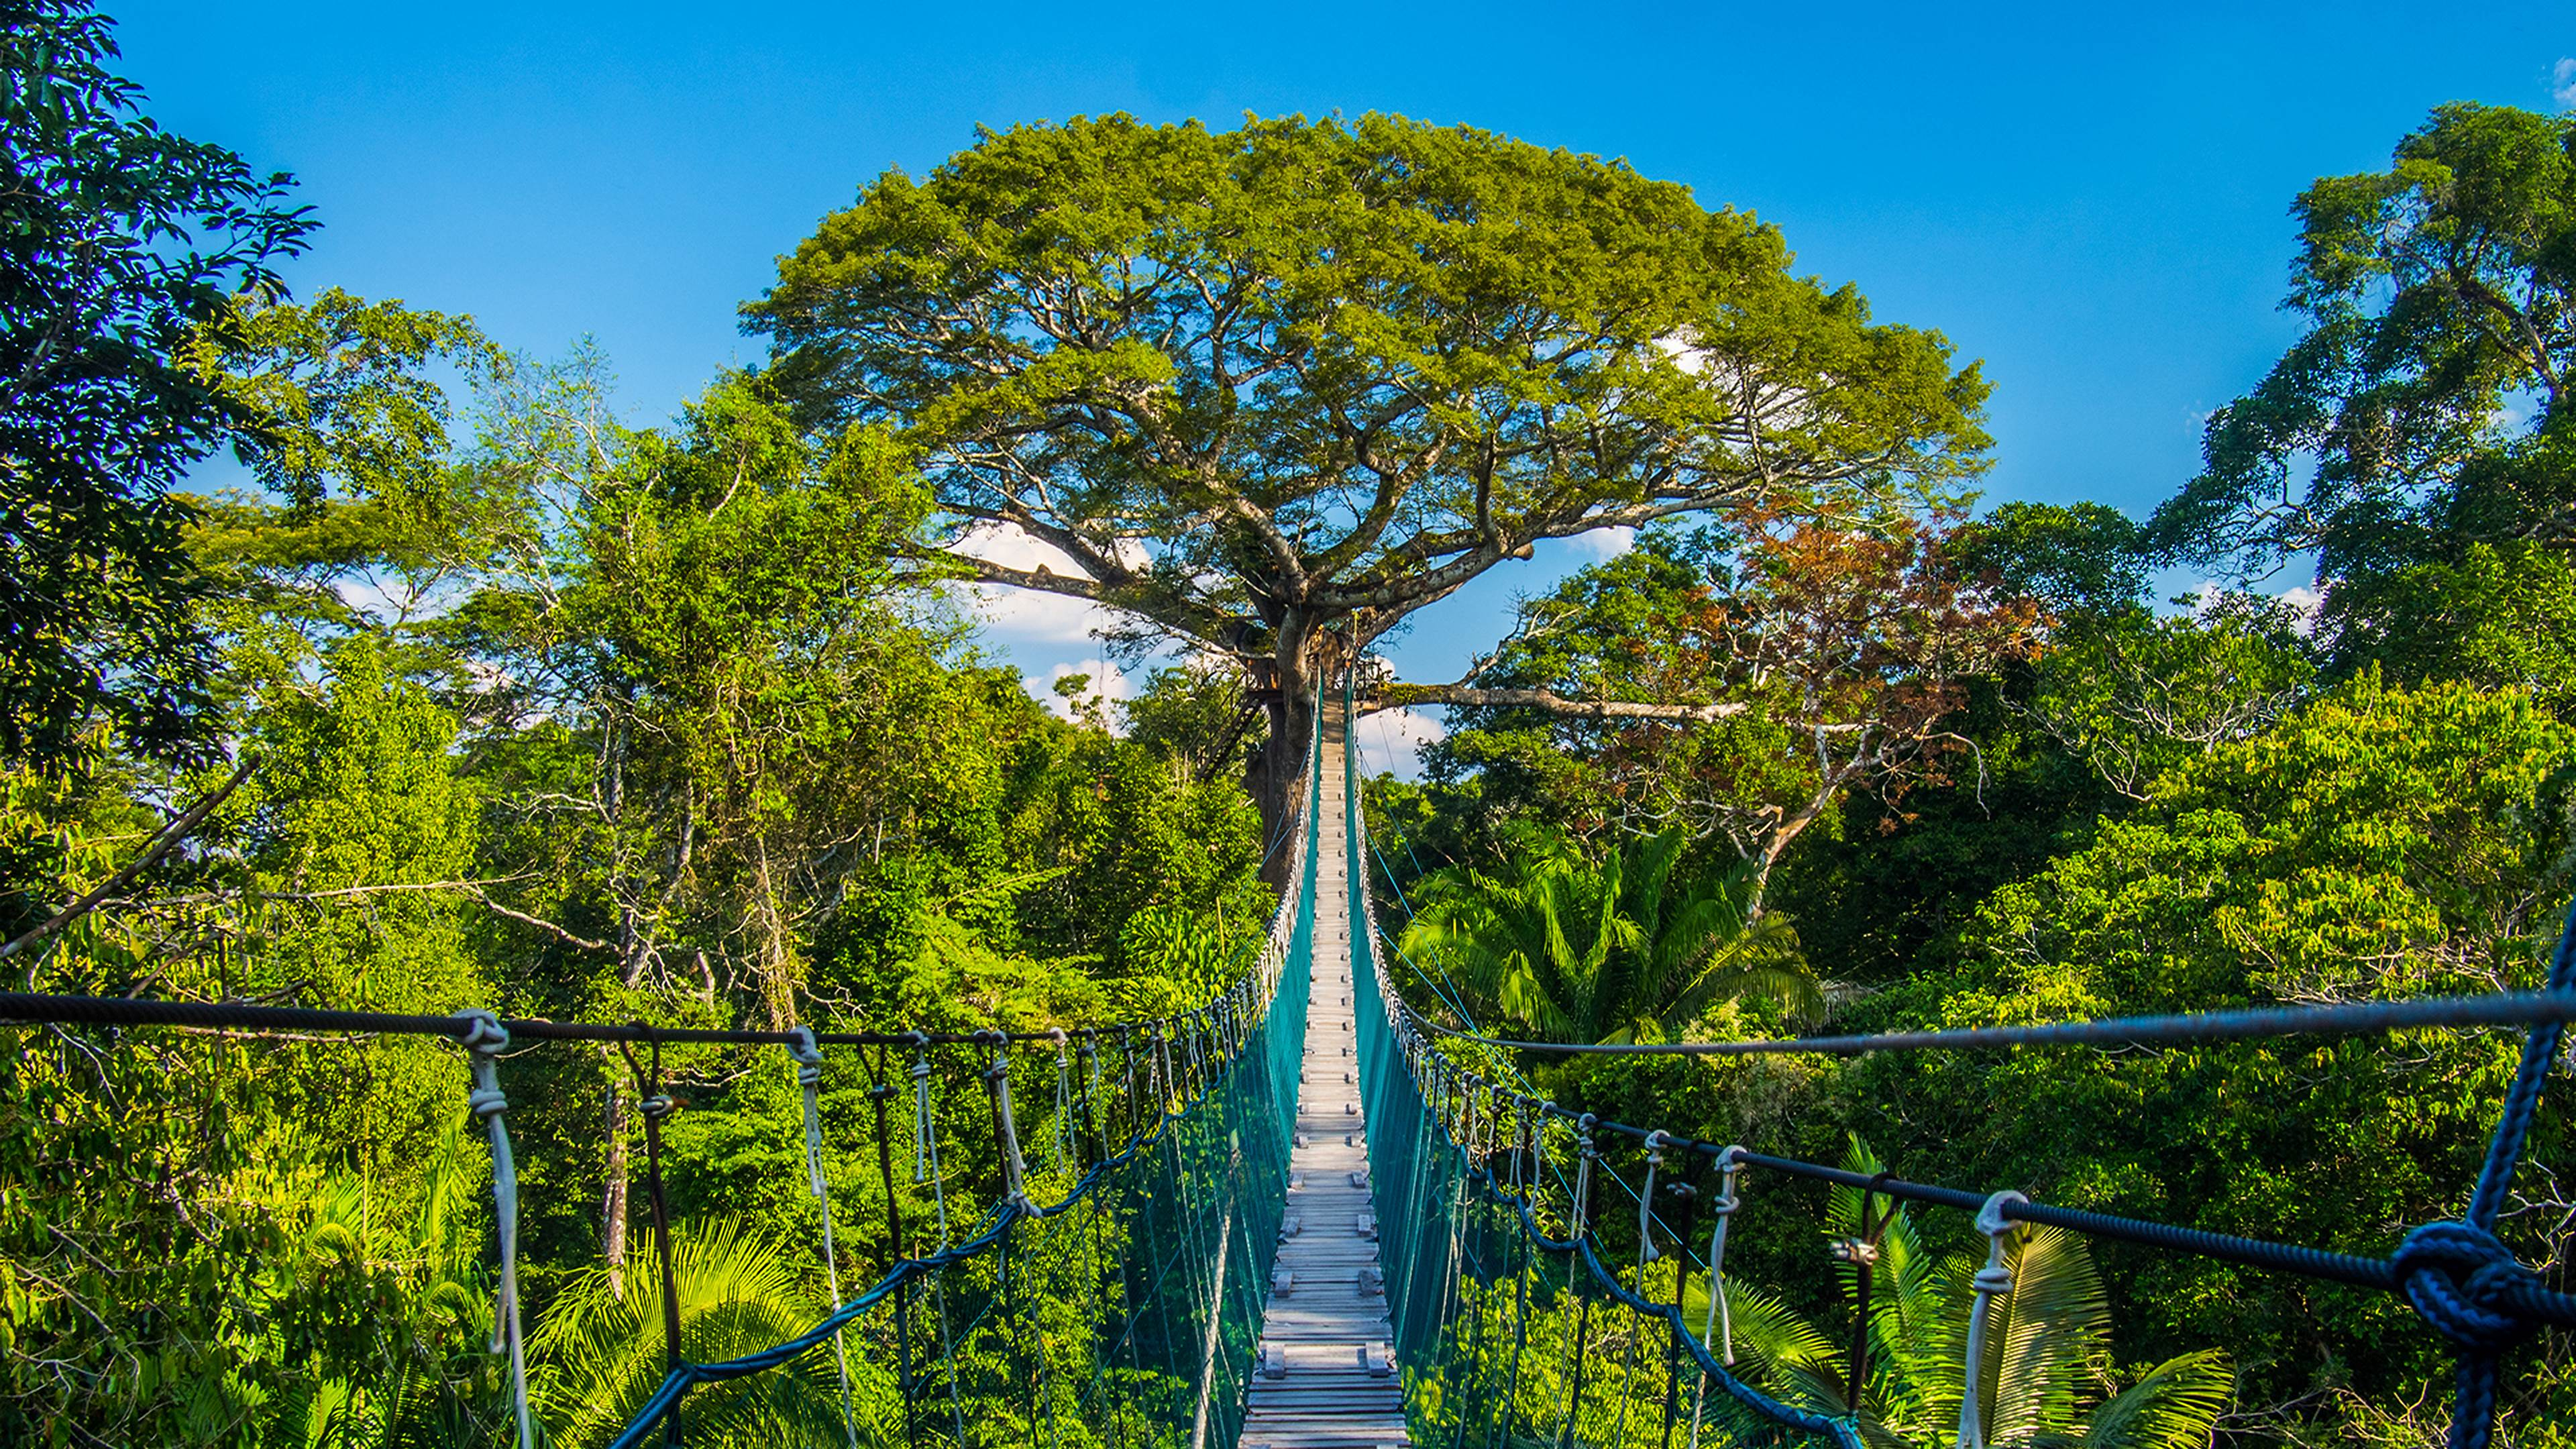
\includegraphics[width=0.3\textwidth]{1.jpeg}
    \end{figure}

    When entering the loop, the $G$-force suddenly acts on the passengers whose maximum value is $6G_s$.

    (In [1], the author states that the maximum $G$-force can reach 12$G_s$. It's not the condition of a perfect circle. Instead, it is possible for a curve with the curvature becomes larger in the process of from top to bottom.)

\end{homeworkProblem}

\pagebreak

\begin{homeworkProblem}

\end{homeworkProblem}

\pagebreak

\begin{homeworkProblem}

    $$
        \phi_1+\phi_2=\phi=\mathrm{const}.\ \ \ \ I=mR^2=\rho R^3\phi.
    $$

    %%若天**力

    $$
        E=\rho R\phi R(1-\cos\varphi)+\frac{1}{2}\rho R^3\phi\dot{\theta}^2
    $$

    $$
        E=\rho R\phi R(1-\cos(\phi_2-\frac{\phi}{2}))+\frac{1}{2}\rho R^3\phi\dot{\phi_2}^2
    $$

    $$
        -\rho\phi Rg^2\sin(\phi_2-\frac{\phi}{2})=\rho R^3\phi\ddot{\phi}_2
    $$

    $$
        \ddot{\phi}_2=-\frac{g}{R}\sin(\phi_2-\frac{\phi}{2})
    $$

    $$
        \mathrm{d}m=\rho R\mathrm{d}\theta
    $$

    $$
        T\mathrm{d}\theta+N+\mathrm{d}mg\cos\theta=\mathrm{d}m\omega^2r
    $$

    $$
        \mathrm{d}T=\mathrm{d}mg\cdot\sin\theta
    $$

    $$
        \Rightarrow\mathrm{d}T=\rho Rg\sin\theta\mathrm{d}\theta+\underbrace{\rho gR\sin(\phi_2-\frac{\phi}{2})}_{\mathrm{constant}}\mathrm{d}\theta
    $$

    $$
        T|_{\phi_2}=T|_{\phi_1}=0
    $$

    \begin{equation}
        T(\theta)=\rho gR(\cos{\phi_2}-\cos\theta)+\rho gR\sin(\phi_2-\frac{\phi}{2})(\phi_2-\theta)
    \end{equation}

    \begin{equation}
        a_{*\&*^\&}=\frac{N}{\mathrm{d}m}=\omega^2r-g\cos\theta-T\frac{\mathrm{d}\theta}{\mathrm{d}m}=\omega^2r-g\cos\theta-\frac{T}{\rho R}
    \end{equation}

    \begin{enumerate}

        \item[\textbf{Case 1:}]

              $\theta=0,\phi_1=0,\phi_2=\phi,T\approx 0$.

        \item[\textbf{Case 2:}]

              $\theta=0,\phi_1=\phi,\phi_2=0,T\approx 0$.

        \item[\textbf{Case 3:}]

              $\theta=0,\phi_1=\frac{\phi}{2},\phi_2=\frac{\phi}{2},T\approx \rho gR(\cos\frac{\phi}{2}-1)$.

              Substituting Eq.(2) into the equation above, we have

              $$
                  a_{\lambda}=\omega^2_{\mathrm{top}}r-g\cos\frac{\phi}{2}
              $$

              $$
                  \Delta \omega^2=\frac{2g}{R}(1-\cos\frac{\phi}{2})
              $$

              $$
                  a_{\lambda}=\omega^2r-2g(1-\cos\frac{\phi}{2})-g\cos\frac{\phi}{2}=\omega^2r-2g+g\cos\frac{\phi}{2}<\omega^2r-g
              $$

              $$
                  \mathrm{d}m=\rho R\mathrm{d}\theta
              $$

              Total length is $\phi$.

              So the accelerate of the two sides is larger than that of the middle.
    \end{enumerate}

\end{homeworkProblem}

\pagebreak

\begin{homeworkProblem}

\end{homeworkProblem}

\pagebreak

\begin{homeworkProblem}

\end{homeworkProblem}

\end{document}